%% ICT Express submission — revised manuscript
%% Format: Elsevier CAS double-column (cas-dc), per the current official
%% Guide for Authors (els-cas-templates is the template bundle the journal
%% currently recommends; LaTeX two-column is permitted for LaTeX submissions).
%% All numbers in tables/figures are \input from script-generated files in
%% ../tables and ../figures; see ../traceability.csv for provenance.

\documentclass[a4paper,fleqn]{cas-dc}

\usepackage[numbers,sort&compress]{natbib}
\usepackage{booktabs}
\usepackage{graphicx}
\usepackage{amsmath}
\usepackage{url}
\usepackage{caption}

\newcommand{\ac}[0]{\ensuremath{ac_1}}

\begin{document}
\let\WriteBookmarks\relax
\def\floatpagepagefraction{1}
\def\textpagefraction{.001}

\shorttitle{What does the LLM actually contribute?}
\shortauthors{Y. Sun and N. Yin}

\title[mode = title]{What Does the LLM Actually Contribute? An Evidence-Constrained
Audit of LLM-Guided Retrieval over Heterogeneous Bilingual RDF Graphs}

\author[1]{Yuxiang Sun}[type=editor,
  orcid=0000-0003-0165-7664]
\credit{Conceptualization, Methodology, Software, Investigation, Writing -- original draft}
\ead{syx921120@gmail.com}
\affiliation[1]{organization={Guangzhou University of Software},
            city={Guangzhou},
            country={China}}

\author[2]{Nan Yin}[orcid=0009-0007-3506-9592]
\credit{Validation, Data curation, Writing -- review \& editing}
\ead{ny@caist.ca}
\affiliation[2]{organization={Canada Advanced Institute of Science and Technology},
            city={Ottawa},
            country={Canada}}

\cortext[1]{Corresponding author.}

\begin{abstract}
Retrieval pipelines that place a large language model (LLM) inside the loop of
knowledge-graph retrieval are usually evaluated end-to-end, making it hard to
attribute measured gains to the model. We re-examine one such pipeline --
LLM-guided entity alignment plus bounded traversal for cross-lingual retrieval
over two heterogeneous RDF graphs (Chinese-labelled schema~X, English-labelled
schema~Y, no \texttt{owl:sameAs}) -- under three controls. First, an
\emph{evidence-constrained} metric (\ac{}) replaces a judge-proxy metric that
was near-tautological with the answer generator. Second, an
\emph{alignment-supervision probe} measures how often the gold URI is already
in the LLM's prompt: on a synthetic bilingual benchmark (49{,}781 triples, 500
queries) this holds for 86.7\% of cross-lingual questions, and success is
0.500 Hits@1 when the gold URI is handed to the 7B planner versus exactly
0.000 when it is not -- the cross-lingual capability is bounded by the supplied
alignment table, not by model knowledge. Third, capability-limited baselines
are replaced by real SPARQL~1.1 (rdflib) and multilingual dense retrieval
(e5-small); real SPARQL recovers two-hop accuracy from 0.000 (legacy) to
0.900, halving the pipeline's apparent advantage (remaining \ac{} lead:
0.772 vs.\ 0.646). Latency is LLM-dominated (seconds vs.\ sub-millisecond
traversal), and localized traversal cuts logical triple access by
$\sim$3 orders of magnitude at no accuracy cost. We conclude what can and
cannot be claimed: an engineering win over weaker baselines on this benchmark,
but cross-lingual ability reflects a supplied lookup table and does not
generalize to self-supervised alignment.
\end{abstract}

\begin{keywords}
knowledge graph \sep RDF retrieval \sep cross-lingual entity alignment \sep large language model \sep evaluation methodology
\end{keywords}

\maketitle

\section{Introduction}\label{sec:intro}
GraphRAG-style pipelines increasingly put an LLM inside the retrieval loop: the
model reads the question, emits a plan (aligned entity URIs, predicate
constraints), and a traversal engine executes the plan over a store. Reported
end-to-end gains are easy to produce and hard to interpret, for three reasons.
The answer generator and the judge may be the same model (inflating every
metric); baselines may be weaker than the real methods they claim to represent;
and when the LLM's prompt already contains ground-truth alignment information,
``the LLM aligned the entity'' may actually mean ``the planner copied a URI it
was given''~\cite{pan2024unifying,barnett2024seven}.

This letter is an evidence-constrained re-evaluation of such a pipeline for
retrieval over two heterogeneous bilingual RDF graphs. The setting is
deliberately synthetic: graph~A uses Chinese labels and schema~X predicates,
graph~B uses English labels and schema~Y predicates, the two graphs describe
the same persons under different URIs, and there is no cross-graph identity
link. We make three contributions:
\begin{enumerate}
\item \textbf{A judge-free, evidence-constrained metric.} \ac{} counts a query
as correct only if the gold entity is ranked first \emph{and} the gold value is
literally present in the retrieved evidence triples; $v_{ic}$ drops the ranking
requirement. Both are computed from saved per-query records and replace a
success metric that was coupled to a deterministic mock answerer.
\item \textbf{An alignment-supervision probe.} For every query we re-derive the
LLM planner's prompt and mark whether the gold URI appears in it verbatim. This
single measurement separates ``the model solved it'' from ``the model selected
what it was shown'' and, to our knowledge, is not routinely reported in
LLM-in-the-loop retrieval evaluations.
\item \textbf{Capability-corrected baselines and cost accounting.} We replace a
``SPARQL'' baseline that never executed SPARQL with real SPARQL~1.1 via
rdflib, and a monolingual hashed-encoder vector baseline with multilingual
dense retrieval (e5-small) plus traversal; we also separate serial service
time, loaded response time, and logical triple access (GSR), which is an
access ratio, not an I/O or memory measurement.
\end{enumerate}
The headline outcome is a demotion, not a promotion: after the corrections,
the pipeline still leads on full-benchmark accuracy (\ac{} $0.772$ vs.\
$0.646$ for real SPARQL, Holm-corrected $p<10^{-7}$), but its cross-lingual
score tracks a supplied lookup table (Section~\ref{sec:probe}), a transliteration
baseline solves every two-character-name query perfectly at $\sim$0.1\,ms
(Section~\ref{sec:baselines}), and the LLM dominates end-to-end latency by
roughly five orders of magnitude over traversal. Although our benchmark is
synthetic, the audit protocol itself is domain-agnostic; Section~\ref{sec:conclusion}
draws out what it implies for three ICT settings with the same structure:
infrastructure metadata management, cross-domain telecom knowledge-graph
integration, and heterogeneous IoT retrieval.

\section{System and benchmark}\label{sec:system}
\textbf{Store.} A deterministic generator builds two rdflib \texttt{Graph}s
with a target of 50{,}000 triples (realized: 49{,}781 triples, 3{,}481
entities, 8{,}218 labels/aliases). Three noise sources are built in: polysemy
(same label, different identities), schema mismatch (synonymous predicates
within each schema), and a cross-lingual naming gap (labels share no
characters across graphs; for two-character names the pair is a romanisation
pair, for three-character names it is not). The generator, queries, seeds,
and all derived records are released with the letter (see the code and data
availability statement), so every number below can be recomputed from the
per-query CSVs alone.

\textbf{Pipeline.} A surface stage matches the query against the label/alias
index in both graphs; an LLM planner (qwen2.5:7b served by Ollama, temperature
0, JSON output, 256-token budget) receives the matched anchors together with
\emph{entity profiles} -- the canonical entity's surface forms in both
languages and all URIs denoting it -- and emits aligned URIs plus predicate
constraints; a localized executor then traverses only the aligned subjects'
triples, expanding one hop along work links when the intent targets work
attributes. The planner is wrapped with a simulated parametric memory whose
coverage (92\%) is an input parameter modelling the long tail an LLM has never
seen; coverage is disclosed rather than measured.

\textbf{Queries.} 500 queries in three families: 200 one-hop attribute
questions, 150 two-hop work-attribute questions, and 150 cross-lingual
questions whose gold counterpart lives only in the other graph. Ground truth
is recorded by the generator, so no answer is invented by a judge.

\textbf{Notation and metrics.} For query $q$, let $R(q)$ be the system's ranked
answer list with rank operator $\rho(q)\in\{1,2,\dots\}$ of the gold entity,
$E(q)\subseteq T$ the evidence triples returned to the answer stage, $v^{*}(q)$
the generator-recorded gold value, and $S(q)\subseteq T$ the triples the
executor logically scanned. Given $n$ queries, the ranking metrics are
\begin{equation}
\mathrm{Hits@1} \;=\; \frac{1}{n}\sum_{q}\mathbf{1}\!\left[\rho(q)=1\right],
\qquad
\mathrm{MRR} \;=\; \frac{1}{n}\sum_{q}\frac{1}{\rho(q)} .
\label{eq:rank}
\end{equation}
The evidence-constrained metrics couple ranking to grounding:
\begin{align}
\ac{}(q) &= \mathbf{1}\!\left[\rho(q)=1 \wedge v^{*}(q)\in E(q)\right],
\label{eq:ac1}\\
v_{ic}(q) &= \mathbf{1}\!\left[v^{*}(q)\in E(q)\right],
\label{eq:vic}
\end{align}
so \ac{} scores a query only when the gold entity is ranked first \emph{and}
the gold value is literally present in the returned evidence; $v_{ic}$ drops
the ranking conjunct. Neither can be satisfied by a judge agreeing with the
answer generator. Logical access is the ratio
\begin{equation}
\mathrm{GSR}(q)\;=\;\frac{|S(q)|}{|T|}\in[0,1],
\label{eq:gsr}
\end{equation}
reported strictly as an access ratio over the store $T$, not as measured
I/O or memory. Accuracy and GSR are aggregated over all 500 queries per
system.

\textbf{Paired tests.} For a binary metric, systems A and B are compared on
the identical query set with McNemar's exact test on the discordant pairs:
writing $b$ for the count with $ac_{1,A}(q)=1,\,ac_{1,B}(q)=0$ and $c$ for the
reverse,
\begin{equation}
p \;=\; 2\!\!\sum_{i=0}^{\min(b,c)}\!\!\binom{b+c}{i}\Big/2^{\,b+c},
\label{eq:mcnemar}
\end{equation}
the two-sided exact tail of $\mathrm{Bin}(b{+}c,\tfrac12)$. For the
continuous GSR we use the Wilcoxon signed-rank statistic on paired
differences $d_q=\mathrm{GSR}_A(q)-\mathrm{GSR}_B(q)$, and Holm's
step-down correction over the family of contrasts within each metric:
$p_{(k)}^{\mathrm{Holm}}=\max_{j\le k}\,(m{-}j{+}1)\,p_{(j)}$ for the ordered
$m$ raw $p$-values.

\section{What the probe shows}\label{sec:probe}
The planner's prompt is built from a ground-truth surface-form table. When the
simulated memory covers an entity, the correct cross-lingual counterpart URI is
inside the prompt. Let $P(q)\subset T$ be the set of URIs that appear in the
planner's prompt for query $q$ (re-derived deterministically from the same
seeds as the main run), $u^{*}(q)$ the gold entity URI, and let
\begin{equation}
g(q)\;=\;\mathbf{1}\!\left[u^{*}(q)\in P(q)\right]
\label{eq:probe}
\end{equation}
mark the \emph{alignment-supervision} condition. The probe estimator simply
stratifies any metric $M$ by this condition,
$\hat{M}_{g=i}=\tfrac{1}{n_i}\sum_{q:\,g(q)=i}M(q)$ with $n_i$ the stratum
size, so a system can be credited with cross-lingual accuracy only on queries
where the gold URI was \emph{not} already shown to it.

Table~\ref{tab:probe} and Figure~\ref{fig:probe} give the outcome split. For
130 of the 150 cross-lingual
queries (86.7\%) the gold URI was in the prompt; the planner achieved Hits@1
$0.500$ on those and exactly $0.000$ on the 20 uncovered queries. The
cross-lingual ability of the pipeline is therefore an upper bound set by the
supplied alignment table, modulated by a near-coin-flip selection rate; it is
not evidence of model-supplied world knowledge. One structural caveat: the
two-hop family's gold answer is a \emph{work} URI reached by traversal, so the
probe does not apply there (marked n/a); those queries succeed through
person alignment plus the two-hop executor, which the ablations confirm
(removing the predicate constraint collapses two-hop \ac{} from 0.933 to 0.000).

{\setlength{\tabcolsep}{3pt}\small%
\begin{tabular}{llrrrr}
\toprule
Query family & Alignment info & $n$ & Hits@1 & MRR & $ac_1$ \\
\midrule
1-hop & absent & 16 & 0.688 & 0.719 & 0.688 \\
1-hop & in prompt & 184 & 1.000 & 1.000 & 0.924 \\
2-hop & n/a & 150 & 0.960 & 0.960 & 0.933 \\
cross-ling. & absent & 20 & 0.000 & 0.000 & 0.000 \\
cross-ling. & in prompt & 130 & 0.500 & 0.750 & 0.500 \\
\bottomrule
\end{tabular}}
\captionof{table}{Alignment-supervision probe: outcomes stratified by whether
the gold URI was present in the planner's prompt.}\label{tab:probe}

\begin{figure}
\centering
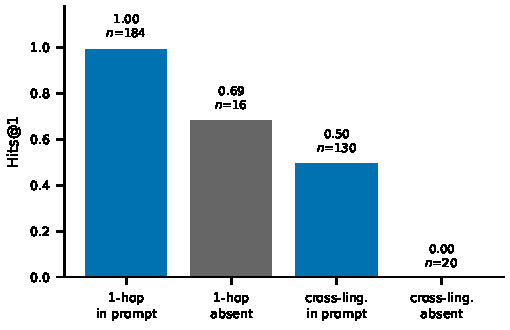
\includegraphics[width=\columnwidth]{../figures/fig3_probe.pdf}
\caption{Alignment-supervision probe. When the gold URI is in the planner's
prompt the 7B planner selects it only half the time on cross-lingual queries;
when it is absent the pipeline never recovers. On one-hop queries the prompt
almost always contains the gold entity (surface matching), and accuracy is
near-perfect.}
\label{fig:probe}
\end{figure}

\section{Capability-corrected baselines}\label{sec:baselines}
The original evaluation compared against (i) a ``SPARQL'' baseline that walked
Python triple patterns without a SPARQL engine and scored 0.000 on two-hop and
cross-lingual families, and (ii) a dense baseline with a monolingual hashed
encoder that scored 0.000 cross-lingually by construction. Neither number
supports a claim about SPARQL or dense retrieval in general.

Table~\ref{tab:main} and Figure~\ref{fig:acc} add three fair systems on the
identical store and query set. \emph{Real SPARQL~1.1} (rdflib engine; two-stage
resolution over \texttt{rdfs:label} and alias predicates, \texttt{VALUES}
push-down, two-hop work pattern) recovers two-hop \ac{} to $0.900$ -- the legacy
number of $0.000$ was an implementation artefact -- and reaches $0.940$ on
one-hop. It scores $0.000$ cross-lingually, which \emph{is} a genuine result:
without \texttt{owl:sameAs} no query can cross the naming gap unaided.
\emph{Multilingual dense retrieval} (e5-small, 8{,}218 passage documents, mean
pooled, L2-normalised) with traversal reaches $0.925$ on one-hop but $0.580$
on two-hop and $0.000$ cross-lingually; removing traversal collapses two-hop
to $0.000$, isolating what the graph step contributes. \emph{Dense without
traversal} reaches only $0.370$ overall: neither head has a cross-lingual
route, so this family of methods is structurally capped on the cross-lingual
third of the benchmark.

\emph{Transliteration.} A small pinyin matcher with identical traversal scores
$0.640/0.613$ on one-hop/two-hop and $0.307$ cross-lingually at $\sim$0.08\,ms
per query (mean, $n=198$). Diagnosis matters more than the headline: its
cross-lingual successes are exactly the 46 two-character-name queries (Hits@1
$1.000$, since those pairs are romanisation pairs by construction) and none of
the 104 three-character-name queries (Hits@1 $0.000$). The $0.307$ is a mixture
fixed by the generator's name-length distribution and must not be read as
evidence that phonetic matching is a strong cross-lingual linker.

Across all contrasts the full system retains a significant lead (all
Holm-corrected $p<10^{-7}$ on \ac{}, $n=500$ paired queries), but the margin
over the strongest fair baseline is $0.772-0.646=0.126$, roughly half of what
the legacy baselines suggested. The in-language ablation also cuts against the
design: dropping the aligner entirely raises one-hop, two-hop and overall
\ac{} to $1.000$, because surface matching plus traversal already suffices
when no cross-graph alignment is required -- the aligner pays a tax
(mis-selection) on the two-thirds of queries that never needed it, connecting
to the known failure mode of retrieving the wrong entity before reasoning
begins \cite{barnett2024seven}.

{\setlength{\tabcolsep}{2.2pt}\scriptsize%
\begin{tabular}{lrrrrrrrr}
\toprule
System & Hits@1 & $ac_1$ & $v_{ic}$ & GSR & $ac_1$(1h) & $ac_1$(2h) & $ac_1$(xl) \\
\midrule
Localized (full) & 0.808 & 0.772 & 0.894 & 3.7e-04 & 0.905 & 0.933 & 0.433 \\
$-$ predicate constr. & 0.520 & 0.520 & 0.656 & 3.1e-04 & 0.975 & 0.000 & 0.433 \\
$-$ localized pruning & 0.808 & 0.772 & 0.894 & 1.0e+00 & 0.905 & 0.933 & 0.433 \\
$-$ aligner & 0.700 & 0.700 & 0.700 & 3.0e-04 & 1.000 & 1.000 & 0.000 \\
$-$ aligner ($k{=}6$) & 0.700 & 0.700 & 0.700 & 3.0e-04 & 1.000 & 1.000 & 0.000 \\
SPARQL 1.1 (rdflib) & 0.646 & 0.646 & 0.700 & 1.6e-01 & 0.940 & 0.900 & 0.000 \\
SPARQL$^{\dagger}$ (no engine) & 0.400 & 0.400 & 0.400 & 1.6e-01 & 1.000 & 0.000 & 0.000 \\
Dense e5 $+$ traversal & 0.544 & 0.544 & 0.672 & 9.0e-04 & 0.925 & 0.580 & 0.000 \\
Dense e5 (no trav.) & 0.370 & 0.370 & 0.418 & 7.8e-04 & 0.925 & 0.000 & 0.000 \\
Vector-GraphRAG$^{\dagger}$ & 0.526 & 0.526 & 0.626 & 9.0e-04 & 0.705 & 0.813 & 0.000 \\
Transliteration & 0.532 & 0.532 & 0.792 & 4.4e-04 & 0.640 & 0.613 & 0.307 \\
\bottomrule
\end{tabular}}
\captionof{table}{Main results at 49{,}781 triples / 500 queries. \ac{} is the
evidence-constrained strict metric; GSR is a logical access ratio, not measured
I/O. $^{\dagger}$Legacy baselines, shown for comparability only; claims rest on
the fair systems. MRR of the full system is 0.874.}\label{tab:main}

\begin{figure}
\centering
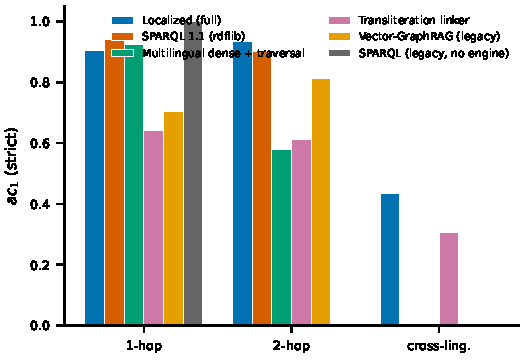
\includegraphics[width=\columnwidth]{../figures/fig2_accuracy.pdf}
\caption{Strict accuracy (\ac{}) per query family. The real SPARQL baseline
recovers two-hop accuracy that the legacy implementation reported as zero;
cross-lingual accuracy is available only to systems that are handed an
alignment table.}
\label{fig:acc}
\end{figure}

\section{Cost structure}\label{sec:cost}
Table~\ref{tab:latency} and Figure~\ref{fig:lat} separate three quantities
that the original evaluation mixed into one column. Serial service time
(cache cleared, warm-up discarded) is dominated by the LLM: the planner costs
$6.7$\,s per query on a stratified 24-query subset, of which $\sim$99.99\% is
model time, while traversal costs fractions of a millisecond. A four-worker
loaded protocol raises the mean to $23.2$\,s ($\sim$3.5$\times$) at the same
0.16 queries/s, confirming that it measures queueing, not parallelism, because
the local Ollama backend serves one request at a time. GSR behaves as
designed: removing localized pruning leaves accuracy identical (\ac{} $0.772$,
$p=1$) while logical access jumps to $1.0$ of the store and traversal time
from $0.19$\,ms to $47.1$\,ms ($\sim$245$\times$), i.e.\ pruning is a pure
cost lever worth $\sim$3 orders of magnitude of logical access, with no
accuracy claim attached.
The scaling sweep confirms the same structure as the store grows. We fit the
log--log model
\begin{equation}
\log \overline{\mathrm{GSR}} \;=\; a + \beta\,\log|T|
\label{eq:fit}
\end{equation}
at sizes $|T|\in\{10^4, 5{\times}10^4, 10^5, 2{\times}10^5\}$: across
10K--200K triples the localized variants' GSR decays with $\beta=-0.98$ to
$-1.02$ ($R^2 \ge 0.999$), i.e.\ logical access stays $O(1)$ in
the number of aligned subjects ($\overline{\mathrm{GSR}}\propto|T|^{-1}$),
while the unpruned variant stays at $1.0$
and the SPARQL systems at $\approx 0.156$ of the store regardless of size
(Fig.~\ref{fig:scaling}). Real SPARQL latency grows linearly
($63$\,ms$\to$$1250$\,ms) whereas the full system stays flat ($\sim$$8.6$\,s,
LLM-dominated).
The real SPARQL engine costs $271$\,ms per query at the 50K operating point
(mean; $146.7$\,ms median) versus $16$\,ms for dense retrieval and $0.08$\,ms for
the transliteration linker, three to five orders of magnitude below the LLM.

\begin{figure}
\centering
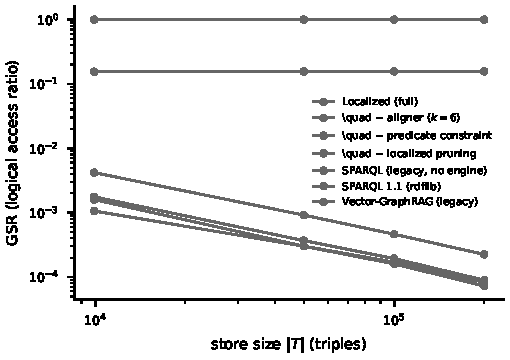
\includegraphics[width=\columnwidth]{../figures/fig4_scaling.pdf}
\caption{GSR (logical access ratio) vs.\ store size, log--log. Localized
variants decay as $|T|^{-1}$; unpruned and SPARQL-family access is
size-proportional.}
\label{fig:scaling}
\end{figure}

{\setlength{\tabcolsep}{2.2pt}\scriptsize%
\begin{tabular}{llrrrrrr}
\toprule
System & Protocol & $n$ & mean & median & P95 & SD & qps \\
\midrule
Localized (full) & serial & 24 & 6703 & 7920 & 9196 & 3166 & 0.1492 \\
\quad $-$ predicate constraint & serial & 24 & 6623 & 7824 & 9023 & 3125 & 0.151 \\
\quad $-$ localized pruning & serial & 24 & 6658 & 7862 & 8980 & 3124 & 0.1502 \\
Localized (full) & 4-worker & 24 & 23216 & 27122 & 32165 & 11392 & 0.1615 \\
\quad $-$ aligner ($k{=}6$) & serial & 198 & 0 & 0 & 0 & 0 & 14421.4 \\
Vector-GraphRAG (legacy) & serial & 198 & 2 & 2 & 2 & 0 & 644.943 \\
SPARQL (legacy, no engine) & serial & 198 & 0 & 0 & 0 & 0 & 14098.3 \\
SPARQL 1.1 (rdflib) & serial & 198 & 271 & 147 & 612 & 177 & 3.6904 \\
Transliteration linker & serial & 198 & 0 & 0 & 0 & 0 & 11479.1 \\
Multilingual dense $+$ traversal & serial & 198 & 16 & 9 & 14 & 43 & 62.2114 \\
\bottomrule
\end{tabular}}
\captionof{table}{Latency protocols. Serial = service time with plan cache
cleared (4 warm-up queries discarded); loaded = 4 workers, which measures
queueing on a single-model backend, not parallelism. $n$ = number of timed
queries; LLM time is measured and included.}\label{tab:latency}

\begin{figure}
\centering
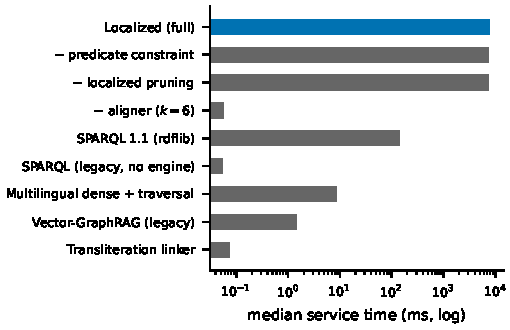
\includegraphics[width=\columnwidth]{../figures/fig5_latency.pdf}
\caption{Median serial service time (log scale). The LLM planner dominates
end-to-end latency by about four orders of magnitude over traversal; the
localized executor and the transliteration linker are sub-millisecond.}
\label{fig:lat}
\end{figure}

\section{Threats to validity and scope}\label{sec:limits}
\textbf{Synthetic data only.} All results come from one generated benchmark.
There is no real ICT/telecommunications deployment, and we make no claim of
one. The benchmark's cross-lingual family tests whether an alignment table was
\emph{provided}, not whether a system can \emph{infer} alignment; systems
without such a table (real SPARQL, dense retrieval) are structurally capped at
zero cross-lingual accuracy here, which is a property of the data design.
\textbf{Simulated memory.} The 92\% coverage parameter controls the
cross-lingual upper bound directly; it is a disclosed input, not a measured
model property. \textbf{One model, one machine.} Latency numbers are specific
to qwen2.5:7b on a local Ollama server and would change with a hosted API.
\textbf{No independent human annotation.} \ac{}/$v_{ic}$ are string-match
checks over saved evidence, not human judgements; the earlier mock-judge
metrics were removed precisely because they could be. \textbf{GSR} counts
logical triple access; it is not measured I/O, memory, or dollars.

\section{Conclusion}\label{sec:conclusion}
With a judge-free metric, a supervision probe, and capability-corrected
baselines, the same benchmark tells a more defensible story: localized
LLM-guided traversal is a genuine cost lever over a real SPARQL engine and
multilingual dense retrieval on full-benchmark accuracy, but its cross-lingual
ability is a function of the alignment table it is given, and a trivial
transliteration matcher already saturates the romanisable subset at four orders
of magnitude lower latency. The actionable lessons are methodological: report
what the prompt contains, judge with metrics the answer generator cannot
influence, and let baselines use the capability they claim to represent.

\textbf{Implications for ICT systems.} The three controls transfer directly
to ICT settings that share the structure studied here -- heterogeneous
schemas, bilingual or multilingual labelling, and no shared identity links.
In \emph{ICT infrastructure metadata management}, asset and catalogue
metadata spread across CRs, inventory and topology systems is exactly the
``two schemas, one entity'' situation; before an LLM planner is credited
with ``resolving'' an asset, the same probe can ask whether the mapped
identifier was already in its prompt. In \emph{cross-domain telecom
knowledge-graph integration}, operator and vendor graphs maintained in
different languages will realistically be bridged by curated alignment
tables rather than \texttt{owl:sameAs}; Eq.~\eqref{eq:probe} gives
integrators a cheap audit of how much of the measured accuracy is inherited
from the table rather than produced by the model. In \emph{heterogeneous
IoT retrieval}, where device, platform, and application ontologies coexist,
the cost findings (LLM seconds vs.\ sub-millisecond traversal; GSR as an
O(1) access ratio) bound where an in-the-loop planner is affordable --
planning is justified only when alignment is genuinely needed and cannot be
replaced by sub-millisecond matching. Future work must move the evaluation
to settings where the alignment table is not handed to the model -- real
public cross-lingual KGs and operational ICT metadata traces -- before any
claim about LLM-supplied cross-lingual knowledge is warranted.

\section*{CRediT authorship contribution statement}
\textbf{Yuxiang Sun:} Conceptualization, Methodology, Software, Investigation,
Writing -- original draft. \textbf{Nan Yin:} Validation, Data curation,
Writing -- review \& editing.

\section*{Declaration of competing interest}
The authors declare that they have no known competing financial interests or
personal relationships that could have appeared to influence the work reported
in this paper.

\section*{Funding}
This work was supported by the 2026 Research Project of Guangzhou University
of Software (grant number KY202649).

\section*{Declaration of generative AI and AI-assisted technologies in the
manuscript preparation process}
During the preparation of this work the authors used an AI assistant in order
to assist with code refactoring, statistical verification and manuscript
editing. After using this tool, the authors reviewed and edited the content as
needed and take full responsibility for the content of the published article.

\section*{Code and data availability}
To support independent verification, the complete audit artefacts are
publicly released under the MIT licence at the repository
\url{https://github.com/CAIST-2026/ict-express-rdf-audit} (release commit
5faa972): (i) the deterministic benchmark generator with its fixed seeds and
the 500 ground-truth queries; (ii) the alignment-supervision probe; (iii) all
baseline and ablation implementations; (iv) the statistical-analysis
scripts; and (v) the per-query result records from which every table, figure,
and number in this letter is derived, together with a provenance index
mapping each reported value to its source file and script. No real operator,
subscriber, or device data is contained in the released artefacts; the
benchmark is synthetic throughout.

\begin{thebibliography}{00}
\bibitem{pan2024unifying}
S. Pan, L. Luo, Y. Wang, C. Chen, X. Wang, X. Wu, Unifying large language
models and knowledge graphs: a roadmap, IEEE Trans. Knowl. Data Eng. 36 (7)
(2024) 3580--3599. https://doi.org/10.1109/TKDE.2024.3305490.
\bibitem{barnett2024seven}
C. Barnett, S. Bhatt, K. Côté, et al., Seven failure points when engineering a
retrieval augmented generation system, in: Proc.\ 3rd International Conference
on AI Engineering (CAiSE), ACM, 2024, pp.\ 1--5.
https://doi.org/10.1145/3726302.3730130.
\bibitem{lewis2020rag}
P. Lewis, E. Perez, A. Piktus, et al., Retrieval-augmented generation for
knowledge-intensive NLP tasks, in: Advances in Neural Information Processing
Systems 33 (NeurIPS), 2020, pp.\ 9459--9474.
\bibitem{rdflib}
G. van Harmelen, S. Schalkwijk, et al., rdflib: a Python library for working
with RDF, version 7.6.0, 2025. https://github.com/RDFLib/rdflib.
\bibitem{e5}
X. Wang, et al., Multilingual E5 text embeddings: a technical report,
arXiv:2402.05672, 2024. https://arxiv.org/abs/2402.05672.
\bibitem{qwen25}
A. Yang, et al., Qwen2.5 technical report, arXiv:2412.15115, 2024.
https://arxiv.org/abs/2412.15115.
\bibitem{mcnemar1947}
Q. McNemar, Note on the sampling error of the difference between correlated
proportions or percentages, Psychometrika 12 (2) (1947) 153--157.
\bibitem{holm1979}
S. Holm, A simple sequentially rejective multiple test procedure, Scand. J.
Stat. 6 (2) (1979) 65--70.
\end{thebibliography}

\end{document}
